% Chapter Template

\section{An agent-based model with optimally behaving agents} % Main chapter title
\label{Model} 
In this section we describe our model, which is derived from \cite{poledna_economic_2019}. We change the household side of the model and add a financial market where agents can trade a market equity fund which pays out dividend of the firms. This stock can also appreciate and depreciate in value. \cite{poledna_economic_2019} use a constant consumption rule where agents consume a fixed part of their expected income. This is a simplification to accurately calibrate the model to the data. However, consumers do not only base their consumption, investment, and savings decisions on current income but also on current investment and savings levels. Therefore, we want to generalize the consumption model within the model of \cite{poledna_economic_2019} by allowing consumption to also depend on liquid and illiquid capital, the interest rates on liquid and illiquid capital and inflation. To clarify, 
\cite{poledna_economic_2019} model consumption $c$, as a constant fraction of income $y$. We generalize this by basing our consumption model on the consumption side of the model of \cite{kaplan_monetary_2018}. By doing so, we relax the constant marginal propensity to consume assumption to the varying marginal propensity to consume. The reasoning behind this is that households with different investment and savings levels have different consumption responses to sudden changes in income. We have chosen for the two asset formulation of \cite{kaplan_monetary_2018}. \cite{kaplan_marginal_nodate} show by comparing a one-asset and two-asset formulation of heterogeneous agent models that the two-asset  formulation is necessary for the theoretical marginal propensity to consume to be close to its empirical counterpart\footnote{A necessary condition for the theoretical marginal propensity to consume to be close to the empirical marginal propensity to consume for a two-asset heterogeneous agent model is that the returns of the liquid and illiquid assets are sufficiently different from each other. \cite{kaplan_marginal_nodate} argue that theory and data give sufficient evidence that this is the case.}.
\subsection{Overview}
Figure \ref{fig:Flow Diagram} shows the overal structure of the model. The economy consists of six sectors namely the household sector, the firm sector, the banking sector, the central bank, the government and the rest of the world. 
\begin{itemize}
    \item Households sell labour to firms in return for wages and invest in firms to claim a share of profits. The households purchase consumption goods of the firms. The households deposits money in the bank or takes a loan from the bank and pays and or receives interest. The firm invest in the equity fund market for which they receive dividend.
    \item Firms produce goods which serve as consumption goods, investment goods, intermediate goods, or as material input. The firms can borrow from the bank and deposit cash reserves at the bank. The firm pays out dividends to the owners of the equity fund.
    \item The bank takes deposits and gives out loans to firms and households. The bank has to adhere to capital requirements and has to do risk assessments of firms that require a loan. Profits are paid out as dividends to households.
    \item The government levies taxes and takes social contributions from households. The government also subsidizes certain sectors and gives out social benefits. Finally, the government also consumes government goods from the firms.
    \item The central bank provides liquidity to the bank in the form of advances or takes deposits of reserves from the bank and pays or receives interest on these. The central bank also sets the policy interest rates.
    \item The rest of the world imports and exports goods on the goods market of the firms.
\end{itemize}
\begin{figure}[h!]
    \centering
    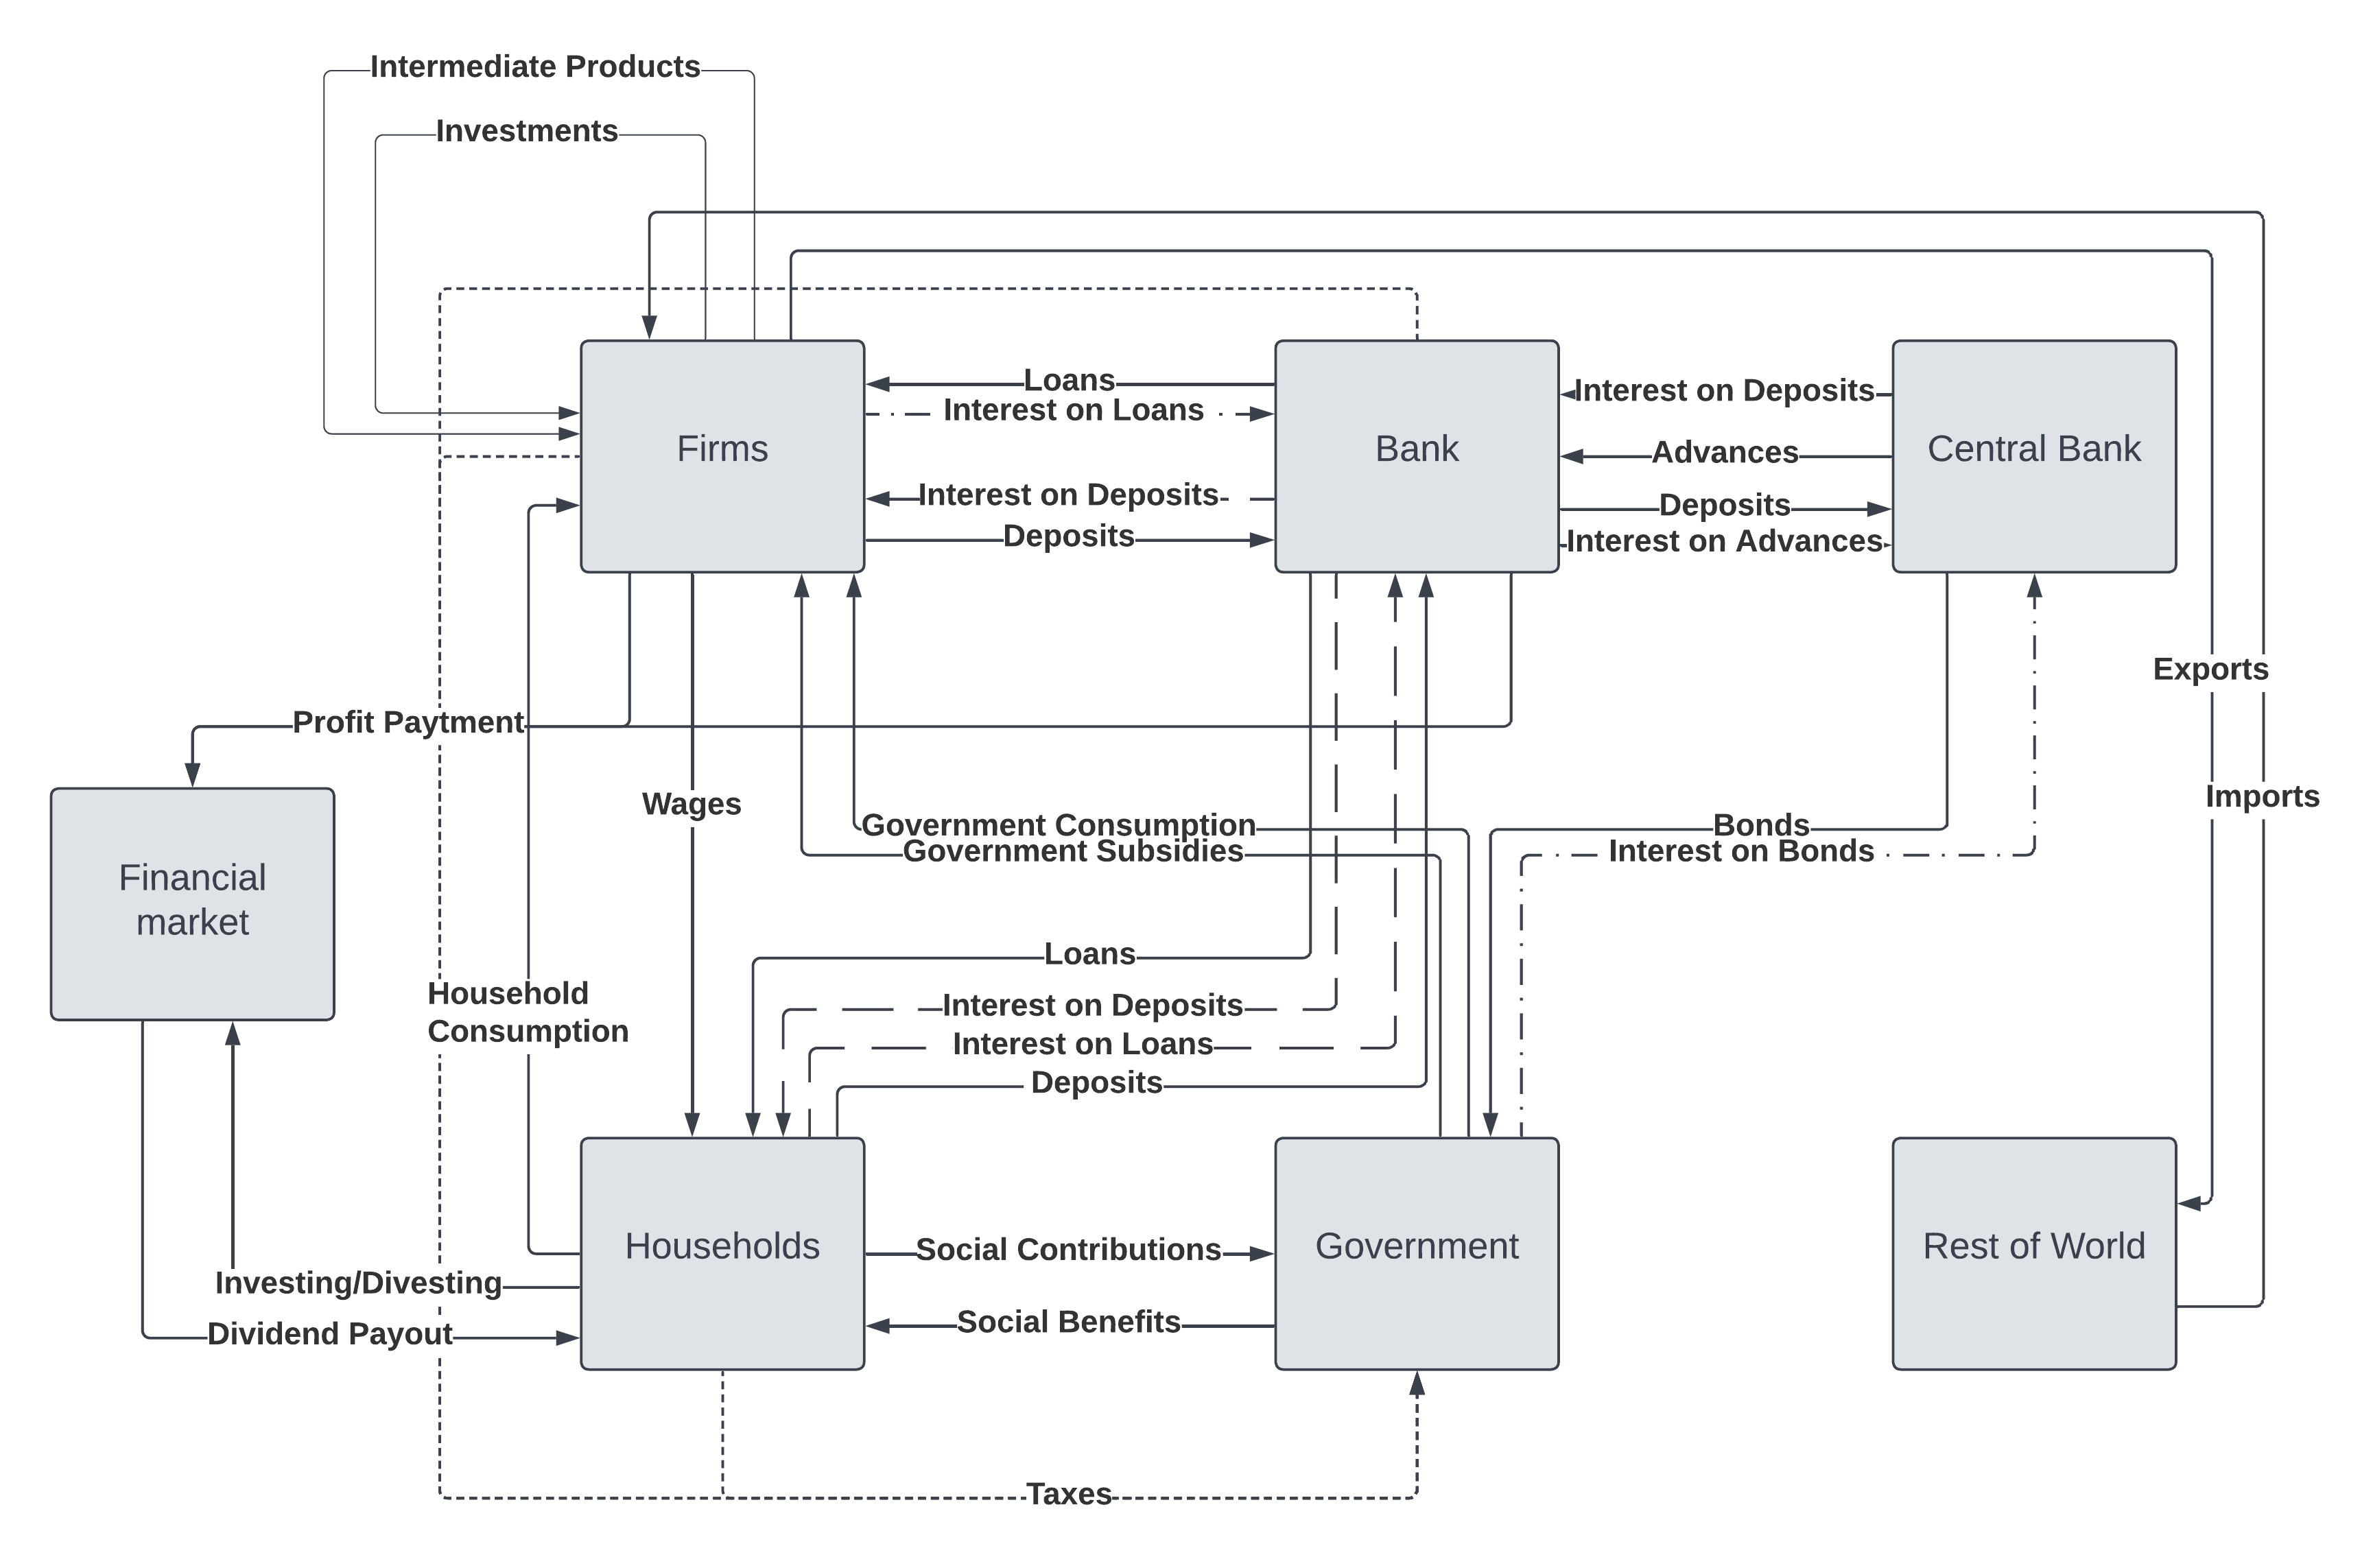
\includegraphics[width=1\textwidth]{figs/Model.png}
    \caption{Flow diagram of the model. The arrow direction indicates flow direction.}
    \label{fig:Flow Diagram}
\end{figure}

\subsection{Households}
As the Dutch Bureau of Statistics registers wealth on household level, we model the household sector on household level. The household sector consists of H households. The income of the household is the sum of the incomes of all people in the household. 

\subsubsection{Household Optimization Problem}
Household income is dependent on the households activity status. If the household $h$ works for firm $i$ in period $t$, then the household receives the wage $w_{h,t}=w_{i,t}$. If the household does not have work and is part of the active households, then the household searches for work by the search-and-matching mechanism on the labour market. This means the household visits firms with open vacancies in a random order. For simplicity, the unemployed person accepts the first job she can find. If she cannot find an open vacancy, she remains unemployed. There are no firing or hiring costs. Fired employees start job searching in the same period. If a household is unemployed she receives unemployment benefits. 
\begin{equation}
    w_{h,t}= \begin{cases}w_{i,t} & \text { if employed by firm } i \\ w_{h,t-1} & \text { otherwise, i.e. if unemployed }\end{cases}\end{equation}
An economic inactive person receives the benefits $sb^{inact}_t$ and does not search for a job.
\begin{equation}
    s b^{\text {inact }}_t=s b^{\text {inact }}_{t-1}\left(1+\gamma^{\mathrm{e}}_t\right)
\end{equation}
Moreover, each household receives other social transfers which are related to family, children, etc. We assume that these benefits are the same for each household:
\begin{equation}
    s b^{\text {other }}_t=s b^{\text {other }}_{t-1}\left(1+\gamma^{\mathrm{e}}_t\right).
\end{equation}
This all together gives the disposable income from labour and social benefits:
\begin{equation}
{\displaystyle 
    Y_{h,t} = \begin{cases}\left(w_{h,t}\left(1-\tau^{\mathrm{SIW}}-\tau^{\mathrm{INC}}\left(1-\tau^{\mathrm{SIW}}\right)\right)+s b^{\text {other }}_t\right) \bar{P}^{\mathrm{HH}}_{t-1} & \text { if employed, } \\ \left(\theta^{\mathrm{UB}} w_{h,t}+s b^{\mathrm{other}}_t\right) \bar{P}^{\mathrm{HH}}_{t-1} & \text { if unemployed, } \\ \left(s b^{\mathrm{inact}}_t+s b^{\mathrm{other}}_t\right) \bar{P}^{\mathrm{HH}}_{t-1} & \text { if not economically active. } \end{cases}}
    \label{eq:income_households}
\end{equation}
We have that $\tau^{INC}$ is the income tax rate, $\tau^{SIW}$ is the rate of social insurance contribution paid by the employee. \\

\subsection{HANK Optimal Consumption Problem}
The household furthermore receives interest on illiquid capital holdings and interest on liquid capital holdings. The interest rate on liquid capital is equal to the firm dividends on the illiquid asset holdings of all agents.
We want to solve the following maximisation problem, which is a simplified discrete version of the household optimisation problem of \cite{kaplan_monetary_2018}. We have removed labour from the consumption problem as this is not available in the CBS micro-database whereas wages are available. Households solve their optimisation problem using partial information about the structure of the economy and hence have boundedly rational expectations for future prices. Essentially, we are using part of the strategy of \cite{krusell_income_1998} who solve an equilibrium model with wealth and income distributions and aggregate uncertainty by letting the agent only use partial information about the distributions summarised by the moments of that distribution. The model is given by:
\begin{equation}
\max _{\{c_{h,t}, d_{h,t}, b_{h,t+1},k_{h,t+1}\}_{t \in \mathbb{N}}} \mathbb{E}_0^* \sum_{t=0}^{\infty} \beta^t u(c_{h,t})
\end{equation}
Such that
\begin{equation}
\begin{aligned}
& p^h_t (1+\tau^{VAT})c_{h,t} = y_{h,t} +\left(1+r_t^b+\mathbb{I}_{\{b_{t+1}<0\}}r_{cc}\right) b_{h,t} -d_{h,t}-\chi(d_{h,t})-b_{h,t+1},\\
& k_{h,t+1}= \left(1+r^k_t-\tau^K\right) k_{h,t}+d_{h,t},\\
& b_{h,t+1}\geqslant -\underline{b}, \quad k_{h,t} \geqslant 0 . 
\end{aligned}
\end{equation}
We moreover have that the cost of adjustment is given by
\begin{equation}
    \chi(d_{h,t})=x_0|d_{h,t}|^{x_1}, \quad x_0, x_1>0.
\end{equation}
Here, $\beta$ denotes the discount rate. $c_{h,t}$ is the consumption of the agent. $b_{h,t}$ denotes liquid assets with borrowing limit $\underline{b}$ and $k_{h,t}$ denote illiquid asset holdings. $d_{h,t}$ is the deposits in illiquid capital. $r^b_t$ denotes the real of the liquid assets at the rate and $r^k_t$ denotes the real rate of illiquid assets. $p^h_t$ is the price of consumption goods. $\tau^{VAT}$ and $\tau^K$ denote value added tax and capital tax respectively. $x_0$ is the size of the transaction cost of investment, and $x_1$ is the convexity of the transaction cost of investment. We choose the constant relative risk aversion utility function given by $\frac{c_{h,t}^{1-\sigma}}{1-\sigma}$. Here, $\sigma$ is the coefficient of risk aversion where $\frac{1}{\sigma}$ is the intertemporal elasticity of substitution. \\

\noindent Agents use adaptive learning of a simple, but optimal AR(1) rule in a complex environment that they do not fully understand. Hence, agents have boundedly rational expectations\footnote{The decision making of the agents is fully rational in the sense that the agents optimize lifetime utility given the constraints and expectations.}. The expectations of the agents can be equivalent to rational expectations if the perceived law of motion is the same as the actual law of motion. In our case, the perceived law of motion and the actual law of motion can never exactly align as the economy is too complex for an AR(1) rule. Each period the agents update the parameters of the perceived law of motion as their information set is updated. Consequently, they update their optimal choice by recalculating the solution of the optimal consumption problem\footnote{We do not believe that in reality agents solve an optimal consumption problem when choosing how much to consume and to save. However, the optimal consumption problem gives a policy function which exhibits several properties that are desirable such as heterogeneous marginal propensities to consume, responding to updates in the information set, and responding to changes in interest rates. We therefore see the policy function generated by the solution of the optimal consumption problem as a good proxy for actual behaviour of an agent. The true causes of the behaviour of a consumer are different than solving an optimization problem}.

\subsubsection{Equity Market}

We assume a very simple capital market where agents can buy and sell shares of the market fund which consists of all firms and the bank. The total number of shares equated to $S = K_0 = \sum_{h=1}^H k_{h,0}$ and is held fixed for the duration of the simulation. We initialize the price of stock at $p_0=1$. When agents invest more or less in the equity market money flows in or out. This appreciates or depreciates the value of the existing stock by changing the price of the market fund. We assume that there is market clearing in the equity market such that the price of the market fund is given by $p_t = K_t / K_0.$ Hence, the number of shares per household is given by $s_{h,t} = \frac{k_{h,t}}{p_t}$. The capital gains return is given by $r^{CG}_t = \frac{p_{t+1}-p_{t}}{p_{t}}$.
The shares payout dividends are the dividends which are paid out by the firms and the bank. The dividend return is calculated as a return on capital which means that $r^{div}_t = \frac{D_t}{K_t}$, where $D_t$ is the sum of total dividend that is paid out by firms and the bank given by \begin{equation*}
    D_t = \underbrace{\sum_{i=1}^I\theta^{\mathrm{DIV}}\left(1-\tau^{\mathrm{FIRM}}\right) \max \left(0, \Pi_{i,t}\right)}_{\text {Dividend payments by firms}} + \underbrace{\theta^{\text {DIV }}\left(1-\tau^{\mathrm{FIRM}}\right) \max \left(0, \Pi_{k,t}\right)}_{\text {Dividend payments by bank}}.
\end{equation*}
The final return on capital $k_{h,t}$ is given by 
\begin{equation}
    r_k^t = r^{CG}_t + r^{div}_t =  \frac{p_{t+1}-p_{t}}{p_{t}} + \frac{D_t}{K_t}.
\end{equation}
\subsubsection{Demanded and Realised Policy Decicisions}
Similar to \cite{poledna_economic_2019} consumers consume goods from different types of companies. The households calculate the demanded consumption and investment budgets by means of the household problem. The consumption budget of the $h$-th household to purchase the $g$-th good is
\begin{equation}
c_{ g,t}^{\mathrm{d}}=\frac{b_g^{\mathrm{HH}} \bar{P}_{g,t} }{\bar{P}^{\mathrm{HH}}_{t-1} } \frac{c_t^{\mathrm{d}}}{1+\tau^{\text{VAT}}},
\end{equation}
where $b_g^{\mathrm{HH}}$ is the consumption coefficient for the gth product of households. $\bar{P}^HH_t$ is the consumer price index and $\bar{P}_{g,t}$ is the producer price index for the principal good $g$, which both are defined in section \ref{Prices}. Once consumers have determined how much they want to consume they will visit firms to purchase goods according to the search-and-matching mechanism. Depending on the inventory and production of a firm either can or cannot completely satisfy the demands of the consumer. Realized consumption of household h is thus determined by: 
\begin{equation}c_t \begin{cases}=\sum_g c_{g,t}^{\mathrm{d}}  & \text { if the consumer successfully realized the consumption plan, and } \\ <\sum_g c_{ g,t}^{\mathrm{d}}  & \text { if all firms visited could not satisfy the consumer's demand }\end{cases}\end{equation}
%Similarly, investment demand by household $h$ for product $g$ net of taxes $\left(d_{g,t}^{\mathrm{d}} \right)$ is then determined by fixed weights $b_g^{\mathrm{CFH}}$ :
%\begin{equation}
%I_{g,t}^{\mathrm{d}}=\frac{b_g^{\mathrm{CFH}} \bar{P}_{g,t-1} }{\sum_g b_g^{\mathrm{CFH}} \bar{P}_{g,t-1} } \frac{I_t^{\mathrm{d}}}{1+\tau^{\text{CF}}}
%\end{equation}
%Similar to the consumption process, realized sales of investment goods purchased by households are determined by the search-and-matching process on the capital goods market:
%\begin{equation}
%I_t \begin{cases}=\sum_g I_{g,t}^{\mathrm{d}} & \text { if the household successfully realized the investment plan, and } \\ <\sum_g I_{g,t}^{\mathrm{d}} & \text { if all firms visited could not satisfy its demand. }\end{cases}
%\end{equation}
When realized consumption and investments are determined, realized savings are also determined by the following equations:
\begin{align}
b_{h,t+1} &= w_{h,t} +\left(1+r_t^b+\mathbb{I}_{\{b_{h,t}<0\}}r_{cc}\right) b_{h,t}-d_{h,t}-\chi (d_{t+1})-p^h_t (1+\tau^{VAT})c_{h,t}\\
    k_{h,t+1} &= \left(1+r^k_t-\tau^K\right) k_{h,t}+d_{h,t+1}
\end{align}



\subsubsection{Expectations}
The economy is too complex to fully understand and therefore agents learn parsimonious but optimal AR(1) forceasting heuristics as in \cite{hommes_behavioral_2014}. They observe past realisations of the price vector and calculate the parameters of the process as econometricians. The perceived laws of motion are given by:

\begin{align}    \mathbb{E}^*_t[r^k_{t+1}]&=\alpha^k_{t} r^k_t +\beta^k_{t}+\epsilon^k_t,\\    \mathbb{E}^*_t[r^b_{t+1}]&=\alpha^b_{t} r^b_t +\beta^b_{t}+\epsilon^b_t, \\
 \mathbb{E}^*_t[\pi_{t+1}] &=\alpha^\pi_t \pi_t+\beta^\pi_{t}+\epsilon^\pi_{t}, \\
\mathbb{E}^*_t[w_{t+1}]&=\alpha^w_{t} w_t +\beta^w_{t}+\epsilon^w_t. 
\end{align}
The parameters $\alpha_{t}^{k}$, $\alpha_{t}^{b}$, $\beta_{t}^{k}$, and $\beta_{t}^{b}$ are re-estimated each period by regressing the interest rate $r_{t}$ on the previous interest rate $r_{t-1}$ means of ordinary least squares for periods $t^\prime \in \{-T,\cdots,t-1\}$. $\epsilon^k_t$ and $\epsilon^b_t$ are random variables with zero mean. The variance is re-estimated every period from past observations. 

\subsubsection{Calculation of the Policy Function}
We use an adapted deep learning approach similar to the approach of \cite{maliar_deep_2021} to calculate the policy functions. \cite{maliar_deep_2021} use an ergodic set to train their neural network, whereas we simply use a sparse grid of the statespace to train our model. The reason for this is that due to the possible nonstationary nature of the agent-based model, the model might leave the ergodic set which assumes a stationary model. The method is as follows: Firstly, we create a theoretical error function $\Xi(\theta)=E_\omega[\xi(\omega ; \theta)]$ which is the sum of the first-order condition of the consumption optimisation problem. As we cannot observe the true error function we train the network on the empirical error function $\Xi^n(\theta)=\frac{1}{n} \sum_{i=1}^n \xi\left(\omega_i ; \theta\right)$. The empirical error function is constructed using the current states of the agents and the future states conditional on the perceived law of motion of the agents. We use Monte Carlo integration to determine the next state of the agents. We then determine the topology of the neural network $\phi(\cdot,\theta)$. We have chosen to use three layers with each 32 nodes and leaky ReLu activation functions with six inputs, which are income, current capital, current savings, current return on capital, current returns on savings, and consumer price $(w, \ k, \ b, \ r^k, \ r^b, p) $ and three outputs, namely current consumption, next-period capital, and next-period savings $(c, \ k, \ b)$. We also randomly fix the initial vector of the coefficients $\theta$. \\

\noindent We use batch stochastic gradient descent with batch size of a hundred agents to let the neural net learn the solution of the consumption optimization problem. This happens as follows: We generate for each agent in the batch an independent draw of the stochastic variables for the next period state according to the agents' perceived law of motion. For instance, we draw $\epsilon^w_t \sim N(0,\sigma^2_{w,t})$ which gives us $w_{i,t+1} = \alpha^w_{t} w_{i,t} +\beta^w_{t}+\epsilon^w_t$. We do this for $r^k_t$ and $r^b_t$, inflation of consumer price $\pi_h$ as well. We can construct the empirical error function using the current state variables $(w_{i,t}, \ k_{i,t}, \ b_{i,t}, \ r^k_t, \ r^b_t, p_t)$, the current decision variables $(c_{i,t}, \ k_{i,t+1}, \ b_{i,t+1}) = \phi(w_{i,t}, \ k_{i,t}, \ b_{i,t}, \ r^k_t, \ r^b_t, \ p_t;\theta)$, the future state variables $(w_{i,t+1}, \ k_{i,t+1}, \ b_{i,t+1}, \ r^k_{t+1}, \ r^b_{t+1}, p_{t+1})$ and future decision variables \\ $(c_{i,t+1}, \ k_{i,t+2}, \ b_{i,t+2}) = \phi(w_{i,t+1}, \ k_{i,t+1}, \ b_{i,t+1}, \ r^k_{t+1}, \ r^b_{t+1} p_{t+1};\theta)$. We collect all these variables in for all the agents in the set $\{\omega_i \}_{i=1}^n$. We compute the gradient of the batch $\nabla \Xi^n(\theta)=\frac{1}{n} \sum_{i=1}^n \nabla \xi\left(\omega_i ; \theta\right)$ and update the coefficients $\theta$ using the following ADAM update scheme of \cite{kingma_adam_2017}. We do this until convergence. The neural net will then solve the first order conditions of optimization problem.\\

\noindent This approach gives us several advantages over classical methods. We can employ machine learning packages which have relatively fast convergence rates in comparison to traditional methods and still have good accuracy \citep{maliar_deep_2021}. We have tried several other methods before which were not fast enough for using in an agent based model such as classical grid methods, projection methods, or sparse adaptive grids \citep{brumm_using_2017}. As we update the expectations of the agent each period we need to recalculate the optimal consumption period each period which necessitates a very fast optimization strategy. Secondly, each period of the simulation of the agent-based model we update the parameters of the perceived law of motion. We can use the parameters of the previous period's neural network as a starting point for the next period's neural network as the next period's solution will be close to the previous period's solution as the parameters of the perceived law of motion update gradually. Therefore, the parameters of the neural network that solves the previous period's optimization problem will be close to the parameters of the neural network that solves the next period's optimization problem. Finally, the neural net does not make use of discretized grids and hence can deal well with a state-space which has changing bounds which we possible are dealing with as the agent-based model is nonstationary.


\subsection{Complex heuristic}
For the third behavioural model, we use a more complex heuristic as a model than the constant consumption rule that is used in the paper of \cite{poledna_economic_2019}. We use the heuristic that is used in \cite{deissenberg_eurace_2008}. This heuristic also has that the agent consumes a constant fraction of their income but also includes wealth in the consumption function. The rule targets a certain wealth-to-income ratio given by $\omega^f$. By having a savings rule which is given by $s_{i,t} = \nu ( \omega^f y^T_{i,t}-TW_{i,t})$. The agent will achieve their target wealth-to-income ratio $\omega^f$ with adjustment speed $\nu$. As a consequence wealth will also follow the same distribution as income but scaled. As savings is given by $s_{i,t} = y_{i,t} - c_{i,t}$, we get that the consumption function is given by $c_{i,t} = (1-\nu \omega^f) Y^T_{i,t} + \nu  TW_{i,t}.$ We assume that agents already have their desired ratio between liquid and illiquid assets and that new savings will be divided between liquid and illiquid assets in the same ratio. This model has no heterogeneous marginal propensity to consume.

The return of capital is simply added to labour income. Hence, we have that income is given by:
\begin{equation}
{\displaystyle 
    Y_{h,t}^{\mathrm{e}}= \begin{cases}\left(w_{h,t}\left(1-\tau^{\mathrm{SIW}}-\tau^{\mathrm{INC}}\left(1-\tau^{\mathrm{SIW}}\right)\right)+s b^{\text {other }}_t\right) \bar{P}^{\mathrm{HH}}_{t-1}\left(1+\pi^{\mathrm{e}}_t\right) +r^k_t K_{h,t} & \text { if employed, } \\ \left.\theta^{\mathrm{UB}} w_{h,t}+s b^{\mathrm{other}}_t\right) \bar{P}^{\mathrm{HH}}_{t-1}\left(1+\pi^{\mathrm{e}}_t\right) +r^k_t K_{h,t}& \text { if unemployed, } \\ \left(s b^{\mathrm{inact}}_t+s b^{\mathrm{other}}_t\right) \bar{P}^{\mathrm{HH}}_{t-1}\left(1+\pi^{\mathrm{e}}_t\right) +r^k_t K_{h,t}& \text { if not economically active. } \end{cases}}
\end{equation}

\section{Simple Heuristic} 
The simple consumption heuristic implies that agents will consume a fixed percentage of their income which is calibrated by the national accounts data. The consumption rule will be given by $c_{i,t} = \phi^C y_{i,t}$. This model has no heterogeneous marginal propensity to consume and does not take differences in wealth into account. We use the same income process as the complex heuristic model.

\begin{figure}
    \centering
    \includegraphics[trim={11cm 5cm 11cm 6cm},clip,width=\textwidth]{figs/policy_funtion.png}
    \caption{Example of optimal consumption function of household agents.
    The parameters for the optimal consumption problem are $\beta=0.98$, $\gamma=1.2$, $x_0=0.01$, and $x_1$=1.1.}
    \label{fig:enter-label}
\end{figure}
       


\subsection{Firms}
We follow \cite{poledna_economic_2019} for the firm sector. The firm sector consists of heterogeneous agents that represent all the Dutch firms for every sector. There are $s \in \{1,\cdots,S\}$ sectors with each $I_s$ firms with total $I=\sum_{i=1}^S I_s$ firms. Each firm $i \in \{1,\cdots,I\}$ produces a principal product $g \in \{1,\cdots,G\}$ using labour, capital, and intermediate inputs from other firms. The demand for the products of the firm $i$ is the sum of the demanded final consumption goods, capital goods, material inputs, and intermediate goods.
\subsubsection{Sales}
The demand of $Q^d_{i,t}$ will be determined only after the firm has determined its price and its production $Y_{i,t}$. Firms experience demand from households and government entities that intend to consume or firms who demand capital or intermediate goods who also act as consumers.\\
\footnotesize
\begin{equation}
Q_{i,t}^{\mathrm{d}} \begin{cases}<Y_{i,t}+S_{i,t-1} & \text { if demand from consumers is smaller than supply from firm } i, \text { and } \\ =Y_{i,t}+S_{i,t-1} & \text { if demand from consumers exactly matches supply from firm } i, \text { and } \\ >Y_{i,t}+S_{i,t-1} & \text { if demand from consumers is larger than supply from firm } i,\end{cases}
\end{equation}
\normalsize
where $S_{i,t-1}$ is the firms inventory of finished goods. Which firm experiences demand is determined by a search-and-matching mechanism. This determines the consumption and supply networks in each period of the model. In each period a consumer visits a number of randomly chosen foreign or domestic firms that sell the good g. The size of a firm and the price that a firm $i$ offers determine the probability that a consumer finds the firm. Two probabilities, one for the lowest price and one for the largest firm, are determined by means of an exponential distribution. Then the average of the two probabilities is used for the search-and-matching process. The probabilities are determined as follows:

\begin{equation}
\begin{aligned}
p r _{i,t}^{\text {price }}  & =\frac{e^{-2 P _{i,t} }}{\sum_{i \in I_{s=g}} e^{-2 P _{i,t} }} \\
p r _{i,t}^{\text {size }}  & =\frac{Y _{i,t} }{\sum_{i \in I_{s=g}} Y _{i,t} } \\
p r _{i,t}^{\text {cum }}  & =\frac{p r _{i,t}^{\mathrm{price}} +p r _{i,t}^{\text {size }} }{2}
\end{aligned}
\end{equation}
Here $p r _{i,t}^{\text {price }} $ is the probability firm $i$ is selected by a consumer due to its offering price. $p r _{i,t}^{\text {size }} $ is the probability firm $i$ is selected by a consumer due to its size. $p r _{i,t}^{\text {cum }} $ is the average probability firm $i$ is selected by a consumer due to its size and its offering price. If the most preferred firm runs out of stock before the consumer has satisfied its demands, the consumer goes to the other firms. If a consumer cannot satisfy its demands for a product $g$ it saves involuntarily. Consequently, actual sales is both determined on demand and supply available and is the minimum of the two quantities:
\begin{equation}
Q_{i,t} = \min \{Y_{i,t} +S_{i,t-1}, Q^d_{i,t}\}
\end{equation}
Excess supply is the difference between production and sales:
\begin{equation}
\Delta S_{i,t} = Y_{i,t}-Q_{i,t}.
\end{equation}
This reflects the firm's expectation error concerning demand. Excess demand is stored as inventory:
\begin{equation}
S_{i,t}=S_{i,t-1}+\Delta S_{i,t}.
\end{equation}
In the next period these goods are available again for sale at the same firm together with the newly produced goods. We assume there is no depreciation of goods.
\subsubsection{Price Setting and Supply}
Expectations for economic growth and inflation are the basis upon which companies make their production and pricing decisions. Firms form expectations for economic growth and inflation using boundedly rational expectations, specifically using AR(1) rules. The expectation formation rule for firms is given by
\begin{equation}
E_t^*[\log \left(Y_{t+1}\right)]=\alpha_{t}^{\mathrm{Y}} \log \left(\sum_i Y_{i,t}\right)+\beta_{t}^{\mathrm{Y}}+\epsilon_{t}^{\mathrm{Y}}. \label{eq:growthar}
\end{equation}

The parameters $\alpha_{t}^{\mathrm{Y}}$ and $\beta_{t}^{\mathrm{Y}}$ are re-estimated each period by regressing aggregate output of firms $\sum_i Y_{i,t^\prime}$ on previous aggregate output of firms $\sum_i Y_{i,t^\prime-1}$ means of ordinary least squares for periods $t^\prime \in \{-T,\cdots,t-1\}$. $\epsilon_{t}^{\mathrm{Y}}$ is a random variable with zero mean. The variance is re-estimated every period from past observations. The growth rate is calculated from aggregate output:
\begin{equation}
\gamma_t^{\mathrm{e}}=\frac{Y_t^{\mathrm{e}} }{\sum_i Y_{i,t}}-1
\end{equation}
The supply choice of the firm is then determined by multiplying the expected growth rate by the previous period's demand for its product:
\begin{equation}
Q_{i,t}^s = Q_{i,t-1}^d(1+\gamma_t^{\mathrm{e}} ).
\end{equation}
Prices are determined by the previous set price, expected inflation and the cost-structure of the firm which is also named cost-push inflation. Hence, the price is given by
\begin{equation}
P_{i,t}=P_{i,t-1} \cdot \underbrace{\left(1+\pi_{i,t}^c\right)}_{\begin{array}{c}
\text { Cost-Push } \\
\text { Inflation }
\end{array}} \cdot \underbrace{\left(1+\pi_t^e\right)}_{\begin{array}{c}
\text { Built-In } \\
\text { Inflation }
\end{array}},
\end{equation}
where

\begin{align}
\begin{split}
\pi_{i,t}^c&=\underbrace{\frac{\left(1+\tau^{S I F}\right) \bar{w}_i}{\bar{\alpha}_i}\left(\frac{\bar{P}_t^{H H}}{P_{i,t}}-1\right)}_{\text {Increase of unit labour costs }}+\underbrace{\frac{1}{\beta_i}\left(\frac{\sum_g a_{s g} \bar{P}_{g,t-1}}{P_{i,t}}-1\right)}_{\text {Increase of unit material costs }}\\
&+\underbrace{\frac{\delta_i}{\kappa_i}\left(\frac{\bar{P}^{C F}_{t-1}}{P_{i,t}}-1\right)}_{\text {Increase of unit capital costs }} \forall i \in I_S .
\end{split}
\end{align}
 $\bar{\alpha}_i$ denotes the average productivity of labour. $\bar{w}_i$ are average gross wages indexed by the consumer price index $\bar{P}_t^{H H} $, and including employers' contribution to social insurance charged with a rate $\tau^{S I F}$. $ \frac{1}{\beta_i} \sum_g a_{s g}$ are unit expenditures (in real terms) on intermediate input by industry $s$ on good $g$ weighted by the average product price index for good $g\left(\bar{P}_{g,t}\right). \delta_i / \kappa_i$ are unit capital costs due to depreciation. $\delta_i$ is the firm's capital depreciation rate and $\kappa_i$ the productivity coefficient for capital. $\bar{P}^{C F}_t $ is the average price of capital goods. Again, expectations on inflation are formed using an AR(1):
\begin{equation}
\mathbb{E}^*_t[\pi_{t+1}] =\alpha^\pi_t \pi_t+\beta^\pi_{t}+\epsilon^\pi_{t}, 
\end{equation}
The parameters $\alpha_{t}^{\\pi}$ and $\beta_{t}^{\pi}$ are re-estimated each period by regressing inflation $\pi_{t^\prime}$ on previous inflation $\pi_{t^\prime}$ means of ordinary least squares for periods $t^\prime \in \{-T,\cdots,t-1\}$. $\epsilon_{t}^{\pi}$ is a random variable with zero mean. The variance is re-estimated every period from past observations. Inflation rate is the log difference of the consumer price index (CPI):
\begin{equation}
\pi_t=\log \left(\frac{\bar{P}_t}{\bar{P}_{t-1}}\right)
\label{eq:expected_inflation}
\end{equation}

where the producer price index is defined as
\begin{equation}
\bar{P}_t=\frac{\sum_i P_{i,t} Q_{i,t}+\sum_m P_{m,t} Q_{m,t}}{\sum_i Q_{i,t}+\sum_m Q_{m,t}}.
\end{equation}
$P_{m,t}$ and $ Q_{m,t}$ are price and sales from foreign producers $m$ respectively. By both incorporating expectations about future cost, inflation and profits and current costs firms lower the probability of becoming bankrupt because of irrational pricing behaviour. Due to the adaptive learning the expectation gap will gradually lower to the actual state of the economy.
\subsubsection{Production}
In every period $t$ each firm $i$ produces output $Y_{i,t}$ in the form of principal product $g$ using labour $N_{i,t}$, intermediate goods and raw materials $M_{i,t}$, and capital $K_{i,t}$. The firms produce by means of a Leontief production function which is given by:
\begin{equation}
Y_{i,t}=\min \left(Q_{i,t}^{\mathrm{S}}, \beta_i M_{i,t}, \alpha_{i,t} N_{i,t}, \kappa_i K_{i,t-1}\right),
\end{equation}
where $\alpha_{i,t}$ is the firm $i$'s labour productivity, $\beta_i$ is the firm's intermediate input productivity and $\kappa_i$ is the firm's capital productivity. Production may be lower than desired production if it cannot obtain enough resources for production.
\subsubsection{Investment}
Every firm $i$ makes an investment decision each period which adjusts next period real capital stock $K_{i,t}$. As today's investment is available to use for production tomorrow capital is durable and sticky. The desired investment in capital stock is given by:
\begin{equation}
    I^d_{i,t} = \frac{\delta_i}{\kappa_i} \min(Q^s_{i,t},\kappa_iK_{i,t}).
\end{equation}
$\delta_i$ is the firm's capital depreciation rate. Capital stock is homogeneous for all firms. Each firm demands $b_g^{CF}I^d_{i,t}$ from firms producing good $g$. Hence, firm $i$'s demand for capital investment in good $g$ is 
\begin{equation}
I^d_{ig,t} = b_g^{CF}I^d_{i,t}.    
\end{equation}
It is possible that firm $i$ cannot realize its capital demand. This is dependent on the search-and-matching process. We have that realized capital investment is given by:
\begin{equation}
I_{I,t} \begin{cases}=\sum_g I_{i g,t}^{\mathrm{d}}  & \text { if the firm successfully realized the investment plan, and } \\ <\sum_g I_{i g,t}^{\mathrm{d}}  & \text { if all firms visited could not satisfy its demand }\end{cases}
\end{equation}
Next period capital stock is determined by realized investment, current capital stock and deprecation due to capital use:
\begin{equation}
    K_{i,t} = K_{i,t-1}-\frac{\delta_i}{\kappa_i}Y_{i,t} +I_{i,t}.
\end{equation}
\subsubsection{Intermediate Inputs}
Intermediate inputs are used by firms for production. Each firm $i$ holds a stock of input goods $M_{i,t}$ in real terms for each good $g$. The firm ensures a positive supply to prevent impeding production. Each period firm $i$ demands intermediate goods such that it can produce its production plan. The desired amount of intermediate goods and raw materials $\Delta M^d_{i,t}$ is given by:
\begin{equation}
    \Delta M^d_{i,t} = \frac{\min \{ Q_{i,t}^s,\kappa_i K_{i,t-1}\}}{\beta_i}
\end{equation}
Moreover, firm $i$ belongs to industry $s$ and consumes intermediate input $g$ according to sector-specific technology coefficients $a_{sg}$ which gives
\begin{equation}
    \Delta M^d_{ig,t} = a_{sg} \Delta M^d_{i,t}, \forall i \in I_s.
\end{equation}
The intermediate inputs also depend on a search-and-matching process which gives:
\begin{equation}
\Delta M_{i,t} \begin{cases}=\sum_g \Delta M_{i g,t}^{\mathrm{d}} & \text { if the firm successfully realized its plan, and } \\ <\sum_g \Delta M_{i g,t}^{\mathrm{d}} & \text { if all firms visited could not satisfy its demand }\end{cases}
\end{equation}
Failure in realizing the firm's production plan results in its production being limited. The evolution of the stock of good $g$ of firm $i$ depends on the usage of the good, the purchasing of the good and the stock of the good of the previous period. This gives us the law of motion:
\begin{equation}
    M_{i,t} =M_{i,t-1} - \frac{Y_{i,t}}{\beta_i} +\Delta M_{i,t}.
\end{equation}
We assume that there is no deprecation of the raw materials as the goods are constantly in use and its stock is being refilled.
\subsubsection{Employment}
Labour $N_{i,t}$ is used as a production input by firm $i$ measured in number of persons employed. The firm demands labour based on its according to desired scale of activity $Q^s_{i,t}$ and average labour productivity $\overline{\alpha}_i$:
\begin{equation}
    N^d_{i,t} = \max \left\{ 1, \operatorname{round}\left(\frac{\min \{ Q_{i,t}^s,\kappa_i K_{i,t-1}\}}{\overline{\alpha}_i}\right) \right\}.
\end{equation}
If a firm demands less than a half-time position, then its demand is rounded down. If it demands more than a half-time position, then demand is rounded up and a new employee is hired. If the operating workforce is higher than is needed, the firm fires $N_{i,t}-N^d_{i,t}$ random employees. If the demand for labour is larger than the current work force, the firm posts labour vacancies:
\begin{equation}
    V_{i,t} = N^d_{i,t} -N_{i,t-1}.
\end{equation}
Vacancies are filled by means of the labour market search-and-matching mechanism.
\begin{equation}
 N_i(t) \begin{cases}=N_i^{\mathrm{d}}(t) & \text { if the firm successfully fills all vacancies, and } \\ <N_i^{\mathrm{d}}(t) & \text { if there are unfilled vacancies. }\end{cases}   
\end{equation}
 Employees can work part-time, full-time, or overtime. This is reflected in the actual productivity of labour $\alpha_{i,t}$. We have that productivity of firm 
$i$ is given by
\begin{equation}
\alpha_{i,t}=\bar{\alpha}_i \min\left(1.5,\frac{\min \left(Q_{i,t}^{\mathrm{S}}, \beta_i M_{i,t-1}, \kappa_i K_{i,t-1}\right)}{N_{i,t} \bar{\alpha}_i}\right).
\end{equation}
The maximum work effort is set to 150 percent of full time employment. Wages are increased or decreased to pay for work efforts relative to normal working hours, such that we have that 
\begin{equation}
w_{i,t}=\bar{w}_i  \frac{\min \left(Q_{i,t}^{\mathrm{S}}, \beta_i M_{i,t-1}, \kappa_i K_{i,t-1}\right)}{N_{i,t} \bar{\alpha}_i}.
\end{equation}
Here, $w_{i,t}$ is the real wage paid by firm $i$. Nominal wages are increased according to inflation.
\subsubsection{External Finance}
It is possible that firms need to finance current o future expenditures by borrowing.  Therefore, each firm forecasts future cash flow $\Delta D_{i,t}^{\mathrm{e}}$, which is equal to the expected change in deposits $D_{i,t}$:
\begin{equation}
    \Delta D_{i,t}^{\mathrm{e}} =\underbrace{\Pi_{i,t}^{\mathrm{e}} }_{\text {Exp. profit }}-\underbrace{\theta L_{i,t-1} }_{\text {Deb instalment }}-\underbrace{\tau^{\mathrm{FIRM}} \max \left(0, \Pi_{i,t}^{\mathrm{e}} \right)}_{\text {Corporate taxes }}-\underbrace{\theta^{\mathrm{DIV}}\left(1-\tau^{\mathrm{FIRM}}\right) \max \left(0, \Pi_{i,t}^{\mathrm{e}} \right)}_{\text {Dividend payout }},
\end{equation}
where
\begin{equation}
    \Pi_{i,t}^{\mathrm{e}} =\Pi_{i,t-1} \left(1+\gamma_t^{\mathrm{e}} \right)\left(1+\pi_t^{\mathrm{e}} \right),
\end{equation}
is expected profit of firm $i$ which is forecasted using previous period profits. $\theta$ is the rate of debt instalments on  firm $i$'s outstanding loans $L_{i,t-1}$. $\tau^{\mathrm{FIRM}}$ is the corporate tax rate. $\theta^{\mathrm{DIV}}$ is the dividend payout ratio. We assume that the dividends are paid out proportionally to the illiquid asset holdings of the households. If a firm cannot use internal finance to pay its expenditure, it will turn to a bank for a loan to cover remaining expected future expenditures:
\begin{equation}
\Delta L_{i,t}^{\mathrm{d}}=\max \left(0,-\Delta D_{i,t}^{\mathrm{e}}-D_{i,t-1}\right)
\end{equation}
Whether the firms gets a loan granted depends on the banks capitalization and the number of firms asking for a loan. If a firm cannot obtain a loan, it might become insolvent.
\subsubsection{Accounting}
\label{Prices}
Firm profits $\Pi_{i,t}$ are an accounting measure. It is defined as revenues from sales plus changes in inventories minus expenditures on labour, material, depreciation, interest payments and taxes
\begin{equation}
\begin{aligned}
\Pi_{i,t}= & \underbrace{P_{i,t} Q_{i,t}}_{\text {Sales }}+\underbrace{P_{i,t} \Delta S_{i,t}}_{\text {Inventory change }}-\underbrace{\left(1+\tau^{\mathrm{SIF}}\right) w_{i,t} N_{i,t} \bar{P}_t^{\mathrm{HH}} }_{\text {Labour costs }} \\
& -\underbrace{\frac{1}{\beta_i} \bar{P}_{i,t} Y_{i,t}}_{\text {Material costs }}-\underbrace{\frac{\delta_i}{\kappa_i} P_{i,t}^{\mathrm{CF}}  Y_{i,t}}_{\text {Depreciation }}-\underbrace{\tau_i^{\mathrm{Y}} P_{i,t} Y_{i,t}-\tau_i^{\mathrm{K}} P_{i,t} Y_{i,t}}_{\text {Net taxes/subsidies on products/production}} \\
& -\underbrace{r_t \left(L_{i,t-1}+\max \left(0,-D_{i,t-1}\right)\right)}_{\text {Interest payments }}+\underbrace{\bar{r}_t  \max \left(0, D_{i,t-1}\right)}_{\text {Interest received }},
\end{aligned}
\end{equation}

 where $r_t$ is the interest rate paid on outstanding loans. The actual prices paid by firm $i$ for intermediate goods and investment in capital goods are  $\bar{P}_{i,t}$ and $P_{i,t}^{\mathrm{CF}}$. These prices are an outcome of the search-and-matching process. Finally, $\bar{P}_t^{\mathrm{HH}} $ is the consumer price index $(\mathrm{CPI})$ :
\begin{equation}
    \bar{P}_t^{\mathrm{HH}} =\sum_g b_g^{\mathrm{HH}} \bar{P}_{g,t}. 
\end{equation}
The parameter $b_g^{\mathrm{HH}}$ is the household consumption coefficient for product $g$ and $\bar{P}_{g,t}$ is the producer price index for the principal $\operatorname{good} g$ :
\begin{equation}
    \bar{P}_{g,t}=\frac{\sum_{i \in I_{s=g}} P_{i,t} Q_{i,t}+P_{m=g,t}  Q_{m=g,t} }{\sum_{i \in I_{s=g}} Q_{i,t}+Q_{m=g,t} } .
\end{equation}
Firm net cash flow is a measure how much liquidity is available for firms to use and is equal to changes in the deposit account:
\begin{equation}
\begin{aligned}
& \Delta D_{i,t}=\underbrace{P_{i,t} Q_{i,t}}_{\text {Sales }}-\underbrace{\left(1+\tau^{\mathrm{SIF}}\right) w_{i,t} N_{i,t} \bar{P}_t^{\mathrm{HH}}}_{\text {Labor costs }}-\underbrace{\bar{P}_{i,t} \Delta M_{i,t}}_{\text {Material costs }} \\
& -\underbrace{\tau_i^{\mathrm{Y}} P_{i,t} Y_{i,t}-\tau_i^{\mathrm{K}} P_{i,t} Y_{i,t}}_{\text {Net taxes/subsidies on products and production }}-\underbrace{\tau^{\mathrm{FIRM}} \max \left(0, \Pi_{i,t}\right)}_{\text {Corporate tax payments }} \\
& -\underbrace{\theta^{\mathrm{DIV}}\left(1-\tau^{\mathrm{FIRM}}\right) \max \left(0, \Pi_{i,t}\right)}_{\text {Dividend payments }}-\underbrace{r\left(L_{i,t-1}+\max \left(0,-D_{i,t-1}\right)\right)}_{\text {Interest payments }} \\
& +\underbrace{\bar{r}_t \max \left(0, D_{i,t-1}\right)}_{\text {Interest received }}-\underbrace{P_{i,t}^{\mathrm{CF}} I_{i,t}}_{\text {Investment costs }}+\underbrace{\Delta L_{i,t}}_{\text {New credit }}-\underbrace{\theta L_{i,t-1}}_{\text {Debt instalment }} . \\
&
\end{aligned}
\end{equation}

Firms have to pay interest on loans and overdrafts (in case $\left.D_{i,t}<0\right)$ at rate $r_t$, which includes the bank's markup rate. When firms have a positive balance on the bank account, i.e. $D_{i,t}>0$, the interest rate received is lower and is equal to the rate set by the central bank.
Firm deposits are equal to deposits plus net cash flow:
\begin{equation}
    D_{i,t}=D_{i,t-1}+\Delta D_{i,t}
\end{equation}
Similarly, debt follows the following law of motion:
\begin{equation}
    L_{i,t}=(1-\theta) L_{i,t-1}+\Delta L_{i,t}
\end{equation}
Firm equity $E_{i,t}$ is computed as a balancing item on the firm's balance sheet taking into account deposits debts, capital and input goods. All goods are accounted for market-to-market:
\begin{equation}
    E_{i,t}=D_{i,t}+\sum_g a_{s g} \bar{P}_{g,t} M_{i,t}+P_{i,t} S_{i,t}+\bar{P}^{\mathrm{CF}}_t  K_{i,t}-L_{i,t} \quad \forall i \in I_s
\end{equation}
$\bar{P}^{\mathrm{CF}}_t $ is defined as the capital goods price index (CGPI) which is given by:
\begin{equation}
    \bar{P}^{\mathrm{CF}}_t =\sum_g b_g^{\mathrm{CF}} \bar{P}_{g,t},
\end{equation}
where $b_g^{\mathrm{CF}}$ is the capital formation coefficient for product $g$.
\subsubsection{Insolvency}
When a firm has negative balance on their deposit account (cash flow insolvent, i.e. $D_{i,t}<0$) and has negative equity value (balance sheet insolvent, i.e. $E_{i,t}<0$) concurrently, then the firm declares bankruptcy. The firm is then replaced by a new firm which enters the market. The real capital stock is taken over from the bankrupt firm at zero costs however the new firm has also to take on part of the liabilities of the old firm.  The remaining liabilities of firm $i$ amount to a fraction $\zeta^{\mathrm{b}}$ of its real capital stock for the new firm as a part of the loans is written off. The remaining liabilities are transferred to the balance sheet of the new firm. In the next period $(t+1)$ liabilities of the new firm $i$ are given by
\begin{equation}
    L_{i,t+1}=\zeta^{\mathrm{b}} \bar{P}_{i,t}^{\mathrm{CF}} K_{i,t}.
\end{equation}
The new firm starts with zero deposits:
\begin{equation}
    D_i(t+1)=0.
\end{equation}
Taking all this together we have that the equity of the new firm $i$ is initialized with
\begin{equation}
    E_i(t+1)=E_{i,t}+\left(L_{i,t}-D_{i,t}-\zeta^{\mathrm{b}} \bar{P}_{i,t}^{\mathrm{CF}} K_{i,t}\right)
\end{equation}

\subsection{Government}
We follow \cite{poledna_economic_2019} for the government sector. The Dutch government is modelled to have two functions: to act as a consumer on the retail market to purchase government consumption and as a redistributive entity that redistributes levied taxes to provide social services to its citizens. Government consumption is assumed to be exogenous.
\subsubsection{Government Consumption}
The government consists out of governmental entities $j \in \{1,\cdots J\}$ which participate in the markets as consumers. These entities represent the state, the province government, the municipalities and social security funds. Governmental demand follows the following rule:
\begin{equation}
    \log \left(C^{\mathrm{G}}_t\right)=\alpha^{\mathrm{G}} \log \left(C^{\mathrm{G}}_{t-1}\right)+\beta^{\mathrm{G}}+\epsilon^{\mathrm{G}}_{t-1} \label{eq:govar}
\end{equation}
where $\epsilon^{\mathrm{G}}_{t-1}$ is a random shock with zero mean and variance $\left(\sigma^{\mathrm{G}}\right)^2$. The total nominal government consumption demand is then uniformly distributed to the $J$ government entities and attributed to goods $g$ :
\begin{equation}
    C_{j,t}^{\mathrm{d}}=\frac{C^{\mathrm{G}}_t \sum_g c_g^{\mathrm{G}} \bar{P}_{g,t-1}\left(1+\pi^{\mathrm{e}}_t\right)}{J}
\end{equation}
and the consumption budget of the $j$-th government entity to purchase the $g$-th good is given by
\begin{equation}
    C_{j g,t}^{\mathrm{d}}=\frac{c_g^{\mathrm{G}} \bar{P}_{g,t-1}}{\sum_g c_g^{\mathrm{G}} \bar{P}_{g,t-1}} C_{j,t}^{\mathrm{d}}
\end{equation}
where $c_g^{\mathrm{G}}$ is the fraction of goods of type $g$ demanded by the government. Realized government consumption is then determined again by the search-and-matching process on the consumption goods market:
$$
C_{j,t} \begin{cases}=\sum_g C_{j g,t}^{\mathrm{d}} & \text { if the government successfully realized the consumption plan, and } \\ <\sum_g C_{j g,t}^{\mathrm{d}} & \text { if all firms visited could not satisfy its demand. }\end{cases}
$$
The government also makes other expenditures such as interest payments, social benefits other than social transfers in kind, and subsidies. The government pays interest at rate $r^G$ on outstanding government debt $L^{\mathrm{G}}_{t-1}$. The government also pays social benefits for inactive households $\left(\sum_{h \in H^{\text {inact }}} s b^{\text {inact }}_t\right)$, social benefits for any household $h\left(\sum_h s b^{\text {other }}_t\right)$, and unemployment benefits for unemployed households $\left(\sum_{h \in H^{\mathrm{U}}(t)} w_{h,t}\right)$. The government also pays subsidies. These are paid to firms via subsidy rates (uniform for each industry, but different across industries) on products and production. These subsidies are incorporated in the net tax rates on products $\left(\tau_i^{\mathrm{Y}}\right)$ and production $\left(\tau_i^{\mathrm{K}}\right)$.
\subsubsection{Government Revenue}
Taxes, social contributions and other transfers from all sectors form the revenue of the government:
\begin{equation}
\begin{aligned}
& Y^{\mathrm{G}}_t=\underbrace{\left(\tau^{\mathrm{SIF}}+\tau^{\mathrm{SIW}}\right) \bar{P}^{\mathrm{HH}}_t\sum_{h \in H^{\mathrm{E}}_t} w_{h,t}}_{\text {Social security contributions }}+\underbrace{\tau^{\mathrm{INC}}\left(1-\tau^{\mathrm{SIW}}\right) \bar{P}^{\mathrm{HH}}_t \sum_{h \in H^{\mathrm{E}}_t} w_{h,t}}_{\text {Labor income taxes }} \\
& +\underbrace{\tau_h^{\mathrm{VAT}} \sum_h C_{h,t}}_{\text {Value added taxes }}+\underbrace{\tau^{\mathrm{INC}}\left(1-\tau^{\mathrm{FIRM}}\right) \theta^{\mathrm{DIV}}\left(\sum_i \max \left(0, \Pi_{i,t}\right)+\max \left(0, \Pi_{k,t}\right)\right)}_{\text {Capital income taxes }} \\
& +\underbrace{\tau^{\mathrm{FIRM}}\left(\sum_i \max \left(0, \Pi_{i,t}\right)+\max \left(0, \Pi_{k,t}\right)\right)}_{\text {Corporate income taxes }}+\underbrace{\tau^{\mathrm{CF}} \sum_h I_{h,t}}_{\text {Taxes on capital formation }} \\
& +\underbrace{\sum_i \tau_i^{\mathrm{Y}} P_{i,t} Y_{i,t}}_{\text {Net taxes/subsidies on products }}+\underbrace{\sum_i \tau_i^{\mathrm{K}} P_{i,t} Y_{i,t}}_{\text {Net taxes/subsidies on production }}+\underbrace{\tau_l^{\text {EXPORT }} \sum_l C_{l,t}}_{\text {Export taxes }} . \\
&
\end{aligned}
\end{equation}
\subsubsection{Government Deficit}
The government deficit (or surplus) is an accounting identity consisting of expenditures minus revenues:
\begin{equation}
\begin{aligned}
\Pi^{\mathrm{G}}_t= & \underbrace{\sum_{h \in H^{\text {inact }}} \bar{P}^{\mathrm{HH}}_t s b^{\text {inact }}_t+\sum_{h \in H^{\mathrm{U}}_t} \bar{P}^{\mathrm{HH}}_t \theta^{\mathrm{UB}} w_{h,t}+\sum_h \bar{P}^{\mathrm{HH}}_t s b_t^{\text {other }}}_{\text {Social benefits and transfers }} \\
& +\underbrace{\sum_j C_P{j,t}}_{\text {Government consumption }}+\underbrace{r^{\mathrm{G}} L_{t-1}^{\mathrm{G}}}_{\text {Interest payments }}-\underbrace{Y_t^{\mathrm{G}}}_{\text {Government revenues }} .
\end{aligned}
\end{equation}
\subsubsection{Government Debt}
The government debt is previous period government debt plus the current deficit:
\begin{equation}
    L^{\mathrm{G}}_t=L^{\mathrm{G}}_{t-1}+\Pi^{\mathrm{G}}_t.
\end{equation}
We assume that the central bank buys all government debt.
\subsection{Bank}
We follow \cite{poledna_economic_2019} for the bank sector. For simplicity, we assume that there is a single bank that represent the entire private financial system. The representative bank takes deposits from households and firms, extends loans to firms, and receives advances from (or deposits reserves at) the central bank.
\subsubsection{Provision of Loans}
The bank extends loans to firms according to a risk assessment of potential borrowers and is subject to minimum capital requirements imposed by the regulator. The bank uses fractional reserve banking, thus the bank is allowed to loan up to a multiple of its equity. The bank is however uncertain about the realized values of its equity due to fundamental uncertainty and thus the bank must forecast future equity value $E_{k,t}^{\mathrm{e}}$ and future outstanding loan value $\sum_{i=1}^I\left(L_{i,t}^{\mathrm{e}}+\Delta L_{i,t}\right)$. The bank has to adhere to a minimum capital requirement coefficient $0<\zeta<1$:
\begin{equation}
\frac{E_{k,t}^{\mathrm{e}}}{\sum_{i=1}^I\left(L_{i,t}^{\mathrm{e}}+\Delta L_{i,t}\right)}=\frac{E_{k,t-1}}{\sum_{i=1}^I\left((1-\theta) L_{i,t-1}+\Delta L_{i,t}\right)} \geq \zeta,
\end{equation}
Therefore, $1/\zeta$ is the maximum allowed leverage for the bank. $\Delta L_{i,t}$ is the realized new loans to firm $i$ in period $t$, which is equivalent to the new credit demanded by firms $\Delta L_{i,t}^{\mathrm{d}}$ if the bank capital requirements are met and the firm borrows within the maximum LTV. When bank capital and leverage requirements are not met, no lending can take place.
Furthermore, the bank forms a risk assessment of a potential default on the part of firm $i$ before extending a loan to it. This risk assessment is based on the borrower's leverage as measured by its loan-to-value ratio, that is the amount of loans over the market value of its capital stock. Thus, the bank will grant a loan to firm $i$ only up to the point where the borrower's leverage (or loan-to-value) ratio after the loan (including overdrafts on deposit accounts), is below a regulated level which is $\zeta^{\mathrm{LTV}}$. Due to fundamental uncertainty, the bank has to form expectations on the value of firm $i$ 's capital stock $\left(K_i^{\mathrm{e}}(t)\right)$ :
\begin{equation}
\frac{L_{i,t}^{\mathrm{e}}+\Delta L_{i,t}}{K_{i,t}^{\mathrm{e}}}=\underbrace{\frac{\overbrace{(1-\theta) L_{i,t-1}}^{=L_{i,t}^{\mathrm{e}}}+\Delta L_{i,t}}{\bar{P}^{\mathrm{CF}}_{t-1}\left(1+\pi_t^{\mathrm{e}}\right) K_{i,t-1}}}_{=K_{i,t}^{\mathrm{e}}} \leq \zeta^{\mathrm{LTV}} .
\end{equation}
Here, $K_{i,t}^{\mathrm{e}}$ denotes the amount of collateral the bank expects a certain firm $i$ to hold at the moment when the firm asks for credit, while $L_{i,t}^{\mathrm{e}}$ is the amount of debt already in the books of the firm.  Altogether, therefore, the amount of new credit extended to firm $i$ by the bank $\left(\Delta L_{i,t}\right)$ depends on the credit demanded by the firm, the bank's risk assessment regarding the default of its potential borrower, and the minimum capital requirements imposed by the regulator:
\begin{equation}
    \Delta L_{i,t} \begin{cases}=\Delta L_{i,t}^{\mathrm{d}} & \text { if the borrower's loan-to-value ratio and capital requirements are satisfied } \\ <\Delta L_{i,t}^{\mathrm{d}} & \text { otherwise. }\end{cases}
\end{equation}
The order of arrival of firms at the bank is random and is important for loan provision. If financially robust (low leverage) firms comes late to the bank, then it may be denied credit if it arrived "too late" (i.e. after other less robust firms). 
\subsubsection{Accounting for Profits and Losses}
The difference between interest revenues from loan provisions (including overdrafts on deposit accounts incurred by firms and households $\left.\left(D_{i, h,t-1}<0\right)\right)$ and costs due to interest payments on deposits held with the bank by firms and households $\left(D_{i, h,t-1}>0\right)$ are the bank's profits. They are computed as follows:
\begin{equation}
    \begin{aligned}
\Pi_{k,t}= & \underbrace{r_t\left(\sum_{i=1}^I L_{i,t-1}+\max \left(0,-D_{i,t-1}\right)+r_t \sum_{h=1}^H \max \left(0,-D_{h,t-1}\right)+\bar{r}_t \max \left(0, D_{k,t-1}\right)\right.}_{\text {Interest received }} \\
& -\underbrace{\bar{r}_t \sum_{i=1}^I \max \left(0, D_{i,t-1}\right)-\bar{r}_t \sum_{h=1}^H \max \left(0, D_{h,t-1}\right)-\bar{r}_t \max \left(0,-D_{k,t-1}\right)}_{\text {Interest payments }}
\end{aligned}
\end{equation}
The bank pays policy rate $\bar{r}_t$ on deposits. This rate is set exogenously by the central bank.  The effective interest rate $r_t$ faced for bank credit or overdrafting is determined by the policy rate $\bar{r}_t$ and a fixed markup $\mu$ :
\begin{equation}
    r_t=\bar{r}_t+\mu
\end{equation}
Bank equity is an accounting identity which is determined by bank profits or losses and is given by
\begin{equation}
    \begin{aligned}
E_{k,t}= & E_{k,t-1}+\Pi_{k,t}-\underbrace{\theta^{\text {DIV }}\left(1-\tau^{\mathrm{FIRM}}\right) \max \left(0, \Pi_{k,t}\right)}_{\text {Dividend payments }} \\
& -\underbrace{\tau^{\mathrm{FIRM}} \max \left(0, \Pi_{k,t}\right)}_{\text {Corporate taxes }}-\underbrace{\sum_{i \in I^{\prime}}\left(L_{i,t}-D_{i,t}-\zeta^{\mathrm{b}} \bar{P}_i^{\mathrm{CF}}(t) K_{i,t}\right)}_{\text {Write-off of bad debt }},
\end{aligned}
\end{equation}
where $I^{\prime}$ is the set of insolvent borrowers. Moreover, the outstanding overdraft of firm $i$ 's deposit account as well as a fraction $\left(1-\zeta^{\mathrm{b}}\right) \bar{P}_{i,t}^{\mathrm{CF}} K_{i,t}$ of loans extended to firm $i$ have to be written off from the bank's balance sheet when firm $i$ is declared bankrupt. The bank's balance sheet consists out of (1) loans to firms (on the asset side); (2) deposits received (on the liability side), (3) equity capital; and (4) (net) central bank reserves held, $D_{k,t}$, or advances obtained by the bank from the central bank: 
\begin{equation}
    D_{k,t}=\sum_{i=1}^I D_{i,t}+\sum_{h=1}^H D_{h,t}+E_{k,t}-\sum_{i=1}^I L_{i,t}
    \label{eq:bankreserves}
\end{equation}
\subsection{Central Bank}
We follow \cite{poledna_economic_2019} for the central bank sector. The central bank (CB) determines monetary policy by setting the policy rate $\overline{r}_t$. The central bank does so taking in consideration implicit inflation and growth targets. It goal is to provide liquidity to the banking system, and to take deposits from the bank in the form of reserves deposited at the central bank. Finally, the central bank also purchases external assets (government bonds).
\subsubsection{Determination of Interest Rates}
A generalized Taylor rule \citep{taylor_discretion_1993} determines the policy rate. We use the same rule as \cite{blattner_towards_2010}, which includes a "growth" rule specification: 
\begin{equation}
    \bar{r}_t=\rho \bar{r}_{t-1}+(1-\rho)\left(r^*+\pi^*+\xi^\pi\left(\pi^{\mathrm{EA}}_t-\pi^*\right)+\xi^\gamma \gamma^{\mathrm{EA}}_t\right)
\end{equation}
where $\rho$ is a measure for gradual adjustment of the policy rate, $r^*$ is the real equilibrium interest rate, $\pi^*$ is the inflation target of the central bank, $ \xi^\pi$ is the weight the central bank puts on inflation targeting and $\xi^\gamma$ the weight placed on economic growth, respectively. Note that the output gap does not enter the equation. Inflation $\left(\pi^{\mathrm{EA}}(t)\right)$ and economic growth $\left(\gamma^{\mathrm{EA}}(t)\right)$ of the monetary union follow an $\mathrm{AR}(1)$  rule given by:
\begin{equation}
    \log \left(1+\pi^{\mathrm{EA}}_t\right)=\alpha^{\pi^{\mathrm{EA}}} \log \left(1+\pi^{\mathrm{EA}}_{t-1}\right)+\beta^{\pi^{\mathrm{EA}}}+\epsilon^{\pi^{\mathrm{EA}}}_{t-1}
\end{equation}
and
\begin{equation}
    \log \left(Y^{\mathrm{EA}}_{t}\right)=\alpha^{\mathrm{Y}^{\mathrm{EA}}} \log \left(Y^{\mathrm{EA}}_{t-1}\right)+\beta^{\mathrm{Y}^{\mathrm{EA}}}+\epsilon^{\mathrm{YA}^{\mathrm{EA}}}_{t-1}
\end{equation}
where
\begin{equation}
    \gamma^{\mathrm{EA}}_t=\frac{Y^{\mathrm{EA}}_t}{Y^{\mathrm{EA}}_{t-1}}-1
\end{equation}
and $\epsilon^{\pi^{\mathrm{EA}}}_{t-1}$ and $\epsilon^{\mathrm{Y}^{\mathrm{EA}}}_{t-1}$ are random shocks with zero mean. $\epsilon^{\pi^{\mathrm{EA}}}_{t-1}$ has variance $\left(\sigma^{\pi^{\mathrm{EA}}}\right)^2$. We assume that the small open economy is part of a monetary union and has no influence on the policy rate. 
\subsubsection{Accounting for Profits and Losses}
The difference between revenues from interest payments on government debt, as well as revenues $\left(D_{k,t}<0\right)$ or costs $\left(D_{k,t}>0\right)$ as a result of the net position in advances or reserves of the banking system is defined as the central bank's profits $\Pi^{\mathrm{CB}}_t$ . Profits are computed by:
\begin{equation}
    \Pi^{\mathrm{CB}}_t=r^{\mathrm{G}} L^{\mathrm{G}}_{t-1}-\bar{r}_t D_{k,t-1} .
\end{equation}
The central bank's equity $E^{\mathrm{CB}}_t$ is an accounting identity dependent on its profits or losses and its past equity. It is computed by:
\begin{equation}
    E^{\mathrm{CB}}_t=E^{\mathrm{CB}}_{t-1}+\Pi^{\mathrm{CB}}_t .
\end{equation}
The following law of motion determines the net creditor/debtor position of the national economy to the rest of the world $\left(D^{\mathrm{RoW}}_t\right)$:
\begin{equation}
    D^{\mathrm{Row}}_t=D^{\mathrm{RoW}}_{t-1}-\underbrace{\left(1+\tau^{\mathrm{EXPORT}}\right) \sum_l C_{l,t}}_{\text {Exports }}+\underbrace{\sum_m P_{m,t} Q_{m,t}}_{\text {Imports }} .
\end{equation}
For instance, a balance of trade surplus $\left(\left(1+\tau^{\mathrm{EXPORT}}\right) \sum_l C_{l,t}>\sum_m P_{m,t} Q_{m,t}\right)$ enters with a negative  sign. This is such as $D^{\mathrm{RoW}}_t$ is on the liability side of the central banks balance sheet. Thus a trade surplus  would reduce national liabilities versus the RoW as it is an inflow of money into  the national economy.  Our financial system is closed via the accounting identity due to inherent stock-flow consistency. This connects the change in the amount of deposits in the banking system to the government deficit (surplus)  and to the balance of trade: 
\begin{equation}
    \begin{aligned}
E^{\mathrm{CB}}_t+D^{\mathrm{RoW}}_t & =L^{\mathrm{G}}(t)-D_{k,t} \\
& =L^{\mathrm{G}}_t-\sum_{i=1}^I D_{i,t}-\sum_{h=1}^H D_{h,t}-E_{k,t}+\sum_{i=1}^I L_{i,t} .
\label{eq:cbequity}
\end{aligned}
\end{equation}
\subsection{Imports and Exports}
We follow \cite{poledna_economic_2019} for the trade with the rest of the world (RoW). Trade of with the RoW is modelled by a set of foreign agents that trade with the domestic economy. Each sector is represented by a single foreign agent which supplies goods on the domestic market for intermediate, capital, and consumption goods. Foreign consumption is also modelled by a single agent for each market. We assume a small open economy setting and hence that demand for export and supply for import is exogenous. Hence, import are constrained by the exogenously set foreign supply. Demand for imports and supply for export is however endogenous. 
\subsubsection{Imports}
Total supply of Imports $Y^I_t$ in real terms follows an AR(1) rule:
\begin{equation}
\log \left(Y^{\mathrm{I}}_t\right)=\alpha^{\mathrm{I}} \log \left(Y^{\mathrm{I}}_{t-1}\right)+\beta^{\mathrm{I}}+\epsilon^{\mathrm{I}}_{t-1}, \label{eq:importsar}
\end{equation}
where $\epsilon^I_{t-1}$ is a random shock with zero mean. A representative foreign firm for each sector imports goods from the rest of the world and supplies them to domestic markets. Thus the $m$-th, $(m\in\{1, \ldots, S\})$, foreign firm representing an industry $s$ imports the principal product $g$
\begin{equation}
    Y_{m,t}=c_{g=s}^I Y^{\mathrm{I}}_t
\end{equation}
where $c_{g=s}^I$ is the fraction of imported goods of type $g$ as part of total imports. Import price is assumed to develop similarly as the average sectoral domestic adjusted for expected inflation.
\begin{equation}
    P_{m,t}=\overline{P}_{g,t-1} (1+\pi^e_t),
\end{equation}
where $m$ produces the principal product g. Sales of imports are equal to the realized demand which is an outcome of the search-and-matching process on the goods markets:
\begin{equation}
    Q_{m,t}=\min \left(Y_{m,t}, Q_{m,t}^d\right)
\end{equation}
where $Q_{m,t}^{\mathrm{d}}$ is subject to the search-and-matching mechanism specifying the demand by consumers from foreign firm $m$ :
\begin{equation}
    Q_{m,t}^{\mathrm{d}} \begin{cases}<Y_{m,t} & \text { if demand from consumers is smaller than supply from foreign firm } m, \\ =Y_{m,t} & \text { if demand from consumers exactly matches supply from foreign firm } m, \text { and } \\ >Y_{m,t} & \text { if demand from consumers is larger than supply from foreign firm } m .\end{cases}
\end{equation}
\subsubsection{Exports}
The export market consists out of foreign consumers $l\in \{1,\cdots,L\}$ which act in the domestic market as consumer. Total demand for export is $C^E_t$ is assumed to be exogenous and follows an AR(1) rule:
\begin{equation}
    \log \left(C^{\mathrm{E}}_t\right)=\alpha^{\mathrm{E}} \log \left(C^{\mathrm{E}}_{t-1}\right)+\beta^{\mathrm{E}}+\epsilon^{\mathrm{E}}_{t-1}, \label{eq:exportsar}
\end{equation}

where $\epsilon^{\mathrm{E}}_{t-1}$ is a random shock with zero mean. The total demand for exports is then uniformly distributed to the $L$ foreign consumers and attributed to goods $g$ :
\begin{equation}
    C_{l,t}^{\mathrm{d}}=\frac{C^{\mathrm{E}}_t \sum_g c_{g,t}^{\mathrm{E}} \bar{P}_{g,t-1}\left(1+\pi^{\mathrm{e}}_t\right)}{L},
\end{equation}
and the demand for exported goods by the $l$-th foreign consumer to purchase the $g$-th good is given by
\begin{equation}
    C_{l g,t}^{\mathrm{d}}=\frac{c_g^{\mathrm{E}} \bar{P}_{g,t-1}}{\sum_g c_g^{\mathrm{E}} \bar{P}_{g,t-1}} C_{l,t}^{\mathrm{d}},
\end{equation}
where $c_g^{\mathrm{E}}$ is the fraction of exports of goods of type $g$. Realized consumption by foreign consumers is again determined by the search-and-matching process on goods markets:
\begin{equation}
    C_{l,t}\begin{cases}=\sum_g C_{l g,t}^{\mathrm{d}} & \text { if the foreign consumer successfully realized the consumption plan, and } \\ <\sum_g C_{l g,t}^{\mathrm{d}} & \text { if all firms visited could not satisfy its demand. }\end{cases}
\end{equation}
\subsection{Macroeconomic Aggregates}
Macroeconomic aggregates are defined the same as in the paper of \cite{poledna_economic_2019}. GDP in the model is calculated by adding the value of all final goods and services produced and purchased by agents in the model in a given period. The nominal GDP and its components of each period $t$ can be measured by three different approaches: (1) production; (2) expenditure based, and (3) income based:
\begin{equation}
    \begin{aligned}
& G D P_t=\underbrace{\sum_i \tau_i^{\mathrm{Y}} P_{i,t} Y_{i,t}+\sum_h \tau^{\mathrm{VAT}} C_{h,t}+\sum_h \tau^{\mathrm{CF}} I_{h,t}+\sum_j \tau^{\mathrm{G}} C_{j,t}+\sum_l \tau^{\mathrm{EXPORT}} C_{l,t}}_{\text {Taxes on products }} \\
& +\underbrace{\sum_i\left(1-\tau_i^{\mathrm{Y}}\right) P_{i,t} Y_{i,t}}_{\text {Total sales of goods and services }}-\underbrace{\sum_i \frac{1}{\beta_i} \bar{P}_{i,t} Y_{i,t}}_{\text {Intermediate inputs }} \text{ (Production Approach)}\\
& =\underbrace{\sum_h\left(1+\tau^{\mathrm{VAT}}\right) C_{h,t}}_{\text {Household consumption }}+\underbrace{\sum_j\left(1+\tau^{\mathrm{G}}\right) C_{j,t}}_{\text {Government consumption }}+\underbrace{\sum_h\left(1+\tau^{\mathrm{CF}}\right) I_{h,t}+\sum_i P_i^{\mathrm{CF}}(t) I_{i,t}}_{\text {Gross fixed capital formation }} \\
& +\underbrace{\sum_i P_{i,t}\left(Y_{i,t}-Q_{i,t}\right)+\bar{P}_{i,t}\left(\Delta M_{i,t}-\frac{1}{\beta_i} Y_{i,t}\right)}_{\text {Changes in inventories }} \text{ (Expenditure Approach)} \\
& +\underbrace{\sum_l\left(1+\tau^{\mathrm{EXPORT}}\right) C_{l,t}}_{\text {Exports }}-\underbrace{\left.\sum_m P_{m,t} Q_{m,t}\right)}_{\text {Imports }} \\
& =\underbrace{\sum_i \tau_i^{\mathrm{Y}} P_{i,t} Y_{i,t}+\sum_h \tau^{\mathrm{VAT}} C_{h,t}+\sum_h \tau^{\mathrm{CF}} I_{h,t}+\sum_j \tau^{\mathrm{G}} C_{j,t}+\sum_l \tau^{\mathrm{EXPORT}} C_{l,t}}_{\text {Taxes on products }} \\
& +\underbrace{\sum_i P_{i,t} Y_{i,t}-\left(1+\tau^{\mathrm{SIF}}\right) \bar{P}^{\mathrm{HH}}(t) N_{i,t} w_{i,t}-\frac{1}{\beta_i} \bar{P}_{i,t} Y_{i,t}-\tau_i^{\mathrm{Y}} P_{i,t} Y_{i,t}-\tau_i^{\mathrm{K}} P_{i,t} Y_{i,t}}_{\text {Gross operating surplus and mixed income }} \\
& +\underbrace{\sum_i\left(1+\tau^{\mathrm{SIF}}\right) \bar{P}^{\mathrm{HH}}(t) N_{i,t} w_{i,t}}_{\text {Compensation of employees }}+\underbrace{\sum_i \tau_i^{\mathrm{K}} P_{i,t} Y_{i,t}}_{\text {Net taxes on production }} \text{ (Income Approach)}\\
&
\end{aligned}
\end{equation}
The GDP deflator is a measure of inflation and is an economy-wide average price of all goods and services produced and sold. All individual prices and sales are determined on the agent level by the search and matching mechanism. In our model, the GDP deflator is defined as nominal GDP divided by real GDP:
\begin{equation}
    G D P \text { deflator }_t=\frac{G D P(t)}{\text { real } G D P(t)},
\end{equation}
where
\begin{equation}
    \begin{aligned}
\text { real } G D P_t= & \sum_i \tau_i^{\mathrm{Y}} Y_{i,t}+\sum_h \tau^{\mathrm{VAT}} \frac{C_{h,t}}{\bar{P}_{h,t}}+\sum_h \tau^{\mathrm{CF}} \frac{I_{h,t}}{\bar{P}_h^{\mathrm{CF}}(t)}+\sum_j \tau^{\mathrm{G}} \frac{C_{j,t}}{\bar{P}_{j,t}} \\
& +\sum_l \tau^{\mathrm{EXPORT}} \frac{C_{l,t}}{\bar{P}_{l,t}}+\sum_i\left(1-\tau_i^{\mathrm{Y}}\right) Y_{i,t}-\sum_i \frac{1}{\beta_i} Y_{i,t} .
\end{aligned}
\end{equation}